\chapter{Dataset}

\section{Scraper}

In order to train our model, we required a substantial amount of data. During our search for a dataset, we discovered that no large dataset for second-hand car prices in the Romanian market existed. Consequently, we decided to develop a scraper.

Throughout this thesis our primary programming language is Python. The choice is based on the need to have great integration with the extensive packages and frameworks in the Python ecosystem. Utilizing \textit{BeautifulSoup4} \cite{bs4}, a package that simplifies web scraping, and \textit{lxml} \cite{lxml} as our parser for improved performance, we successfully obtained a dataset of 46,893 advertisements. This dataset includes various parametric data, detailed descriptions, and ten images for each post.

Our primary tool for handling the data obtained from scraping, formatting, and cleaning it for analysis, inference, and preprocessing is \textit{Pandas} \cite{pandas}, a versatile library for data manipulation and analysis. Pandas offers robust data structures and a wide range of functions, simplifying the efficient handling of both numerical and categorical data.

\subsection{Scraping Strategy}

After analyzing the major players in Romania's second-hand car market, we identified Autovit and OLX as the leading platforms. Both platforms command significant market shares. However, we selected Autovit as our primary data source. This decision was influenced by Autovit's requirement for more mandatory data fields when creating an advertisement. These fields provide richer information for our predictive model, making the data more valuable compared to OLX. Additionally, scraping both platforms would have introduced complexities due to potential duplicate entries, which could compromise the integrity and usability of our dataset.

One of the initial strategic decisions was to focus exclusively on listings of undamaged cars. We chose this approach because predicting prices for damaged cars introduces significant complexity, given the variability in the car's usability, visual aspect, and functional status.

\subsection{Scraping Implementation}

The scraping process was divided into four distinct stages, each designed to collect and integrate data from the Autovit platform. Below is a detailed explanation of each stage:

\begin{enumerate}
    \item \textbf{URL Collection}: In the first stage of our scraping process, our primary objective was to gather URLs that link to individual car advertisements where the needed details are present. To achieve this, we navigated through all accessible pages of the website, with a focus on the latest 500 pages due to the site's pagination limits. We employed a custom script to automate the collection of these URLs, which served as entry points for more detailed data extraction in subsequent stages. To enhance the efficiency and relevance of our data collection, the script was designed to identify and ignore duplicate advertisements during this initial gathering phase.
    \item \textbf{Detailed Ad Scraping}: Once the URLs were collected, the second stage involved extracting detailed information from each listed advertisement. This included gathering essential parametric data such as manufacturer, model, year, and price. Additionally, we extracted information on custom options like heated seats or infotainment systems, as well as the full descriptions of each advertisement, providing deeper insights into each vehicle’s features and condition. \hyperref[fig:scraping-details]{Figure 3.1} showcases the website components from which these details were scraped.
    \item \textbf{Image Download}: The third stage focuses on downloading images from the advertisements. Considering the significant storage and processing requirements of handling large volumes of images, we strategically limited the download to the first ten images per advertisement. This decision was based on a balance between obtaining sufficient visual data (over 160GB in images) for analysis and maintaining manageable data volumes.
    \item \textbf{Data Integration}: The final stage involved integrating newly scraped data with the existing dataset. Since the scraper was scheduled to run weekly, each new cycle added fresh data to our collection.
\end{enumerate}

\begin{figure}
    \centering
    \begin{subfigure}{\linewidth}
        \centering
        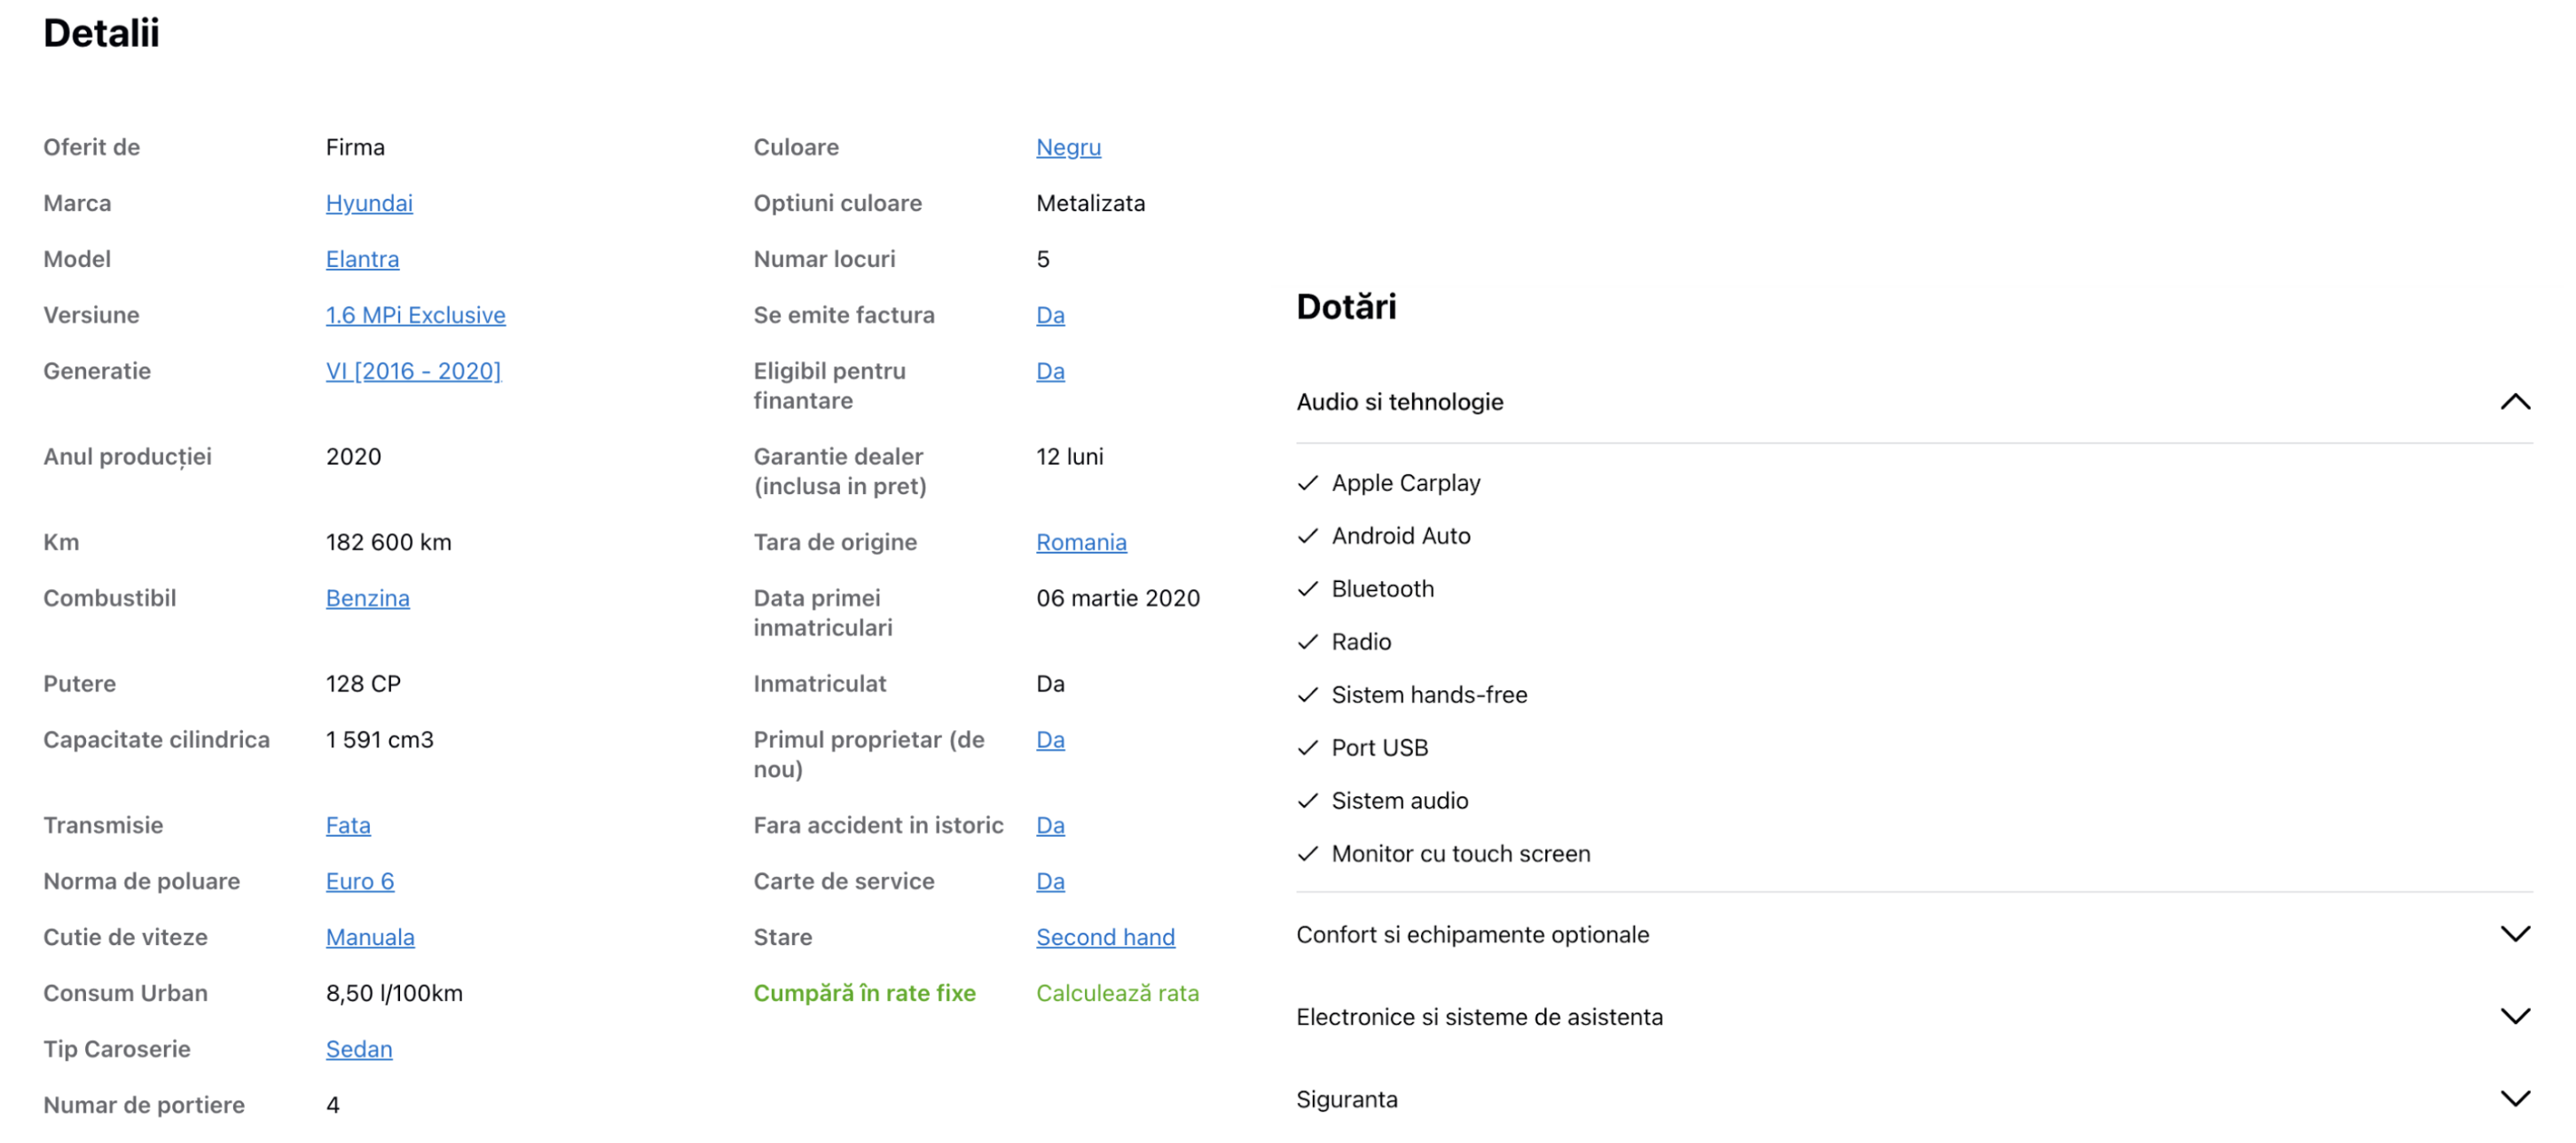
\includegraphics[width=\linewidth]{images/priceprediction/data/Screenshot 2024-05-28 at 21.33.53.png}
    \end{subfigure}
    \hfill
    \begin{subfigure}{\linewidth}
        \centering
        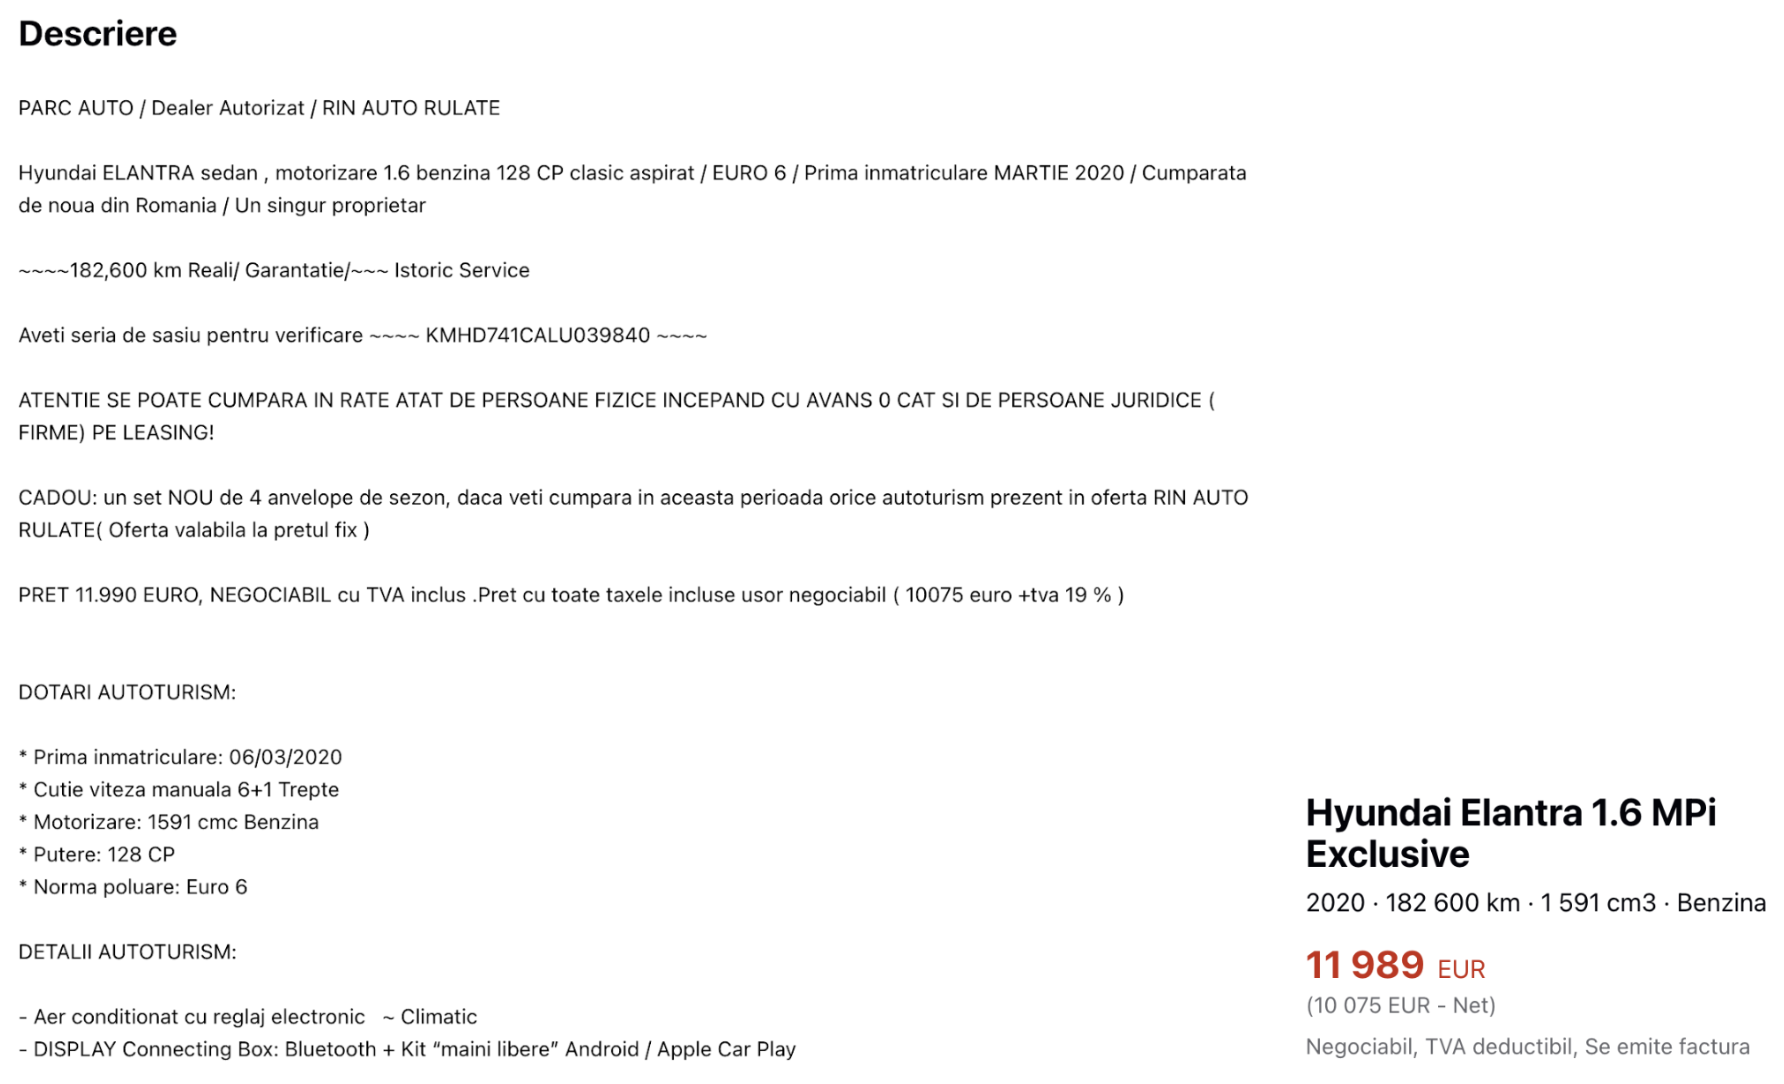
\includegraphics[width=\linewidth]{images/priceprediction/data/Screenshot 2024-05-28 at 21.39.39.png}
    \end{subfigure}
    \caption{Scraping Details}
    \label{fig:scraping-details}
\end{figure}

These stages formed a robust framework for our web scraping operations, ensuring efficient data collection and ongoing updates to support our machine learning model for car price prediction.

\subsection{Challenges and Solutions}
During the development and operation of our web scraping system, we encountered several challenges that required attention to ensure the effectiveness and efficiency of our data collection process. Here are the key challenges and the strategies we implemented to overcome them:

\begin{itemize}
    \item \textbf{Processing Speed}: Initially, the data scraping process was slow, hindering our ability to gather data efficiently. To address this, we implemented a multithreaded approach. This allowed us to execute multiple scraping operations in parallel, significantly reducing the time required to navigate through and download data from web pages. The enhancement in speed enabled us to handle larger volumes of data within shorter time frames, making our data collection process much more efficient.

\begin{lstlisting}
with ThreadPoolExecutor() as executor:
    futures = []

    for index, row in df.iterrows():
        future = executor.submit(process_row, df, index, row)
        futures.append(future)

    for future in futures:
        future.result()
\end{lstlisting}

    \item \textbf{Network Errors}: We frequently encountered network errors and timeouts, which disrupted the scraping process. To mitigate this, we implemented an automatic retry mechanism. Each failed request was automatically retried up to five times before the system moved on to the next task. This approach significantly reduced data loss due to transient network issues and ensured a higher success rate in data retrieval.

    \item \textbf{Limited Data Availability}: The Autovit platform restricts access to only the last 500 pages of listings, containing around 15,000 advertisements, which was insufficient for building a robust dataset. To overcome this limitation, we developed a recurring scraping strategy. By running our scraper weekly, we were able to continuously capture new listings as they were posted, adding approximately 5,000 new advertisements to our dataset each week. 
\end{itemize}

These solutions significantly improved our dataset, enabling us to construct a larger and more up-to-date dataset that effectively supports our car price prediction model.

\subsection{Ethical and Legal Considerations}
We ensured compliance with web scraping legal standards and Autovit’s terms of service \cite{AutovitTerms}, particularly regarding data privacy and usage policies.

\paragraph{The structure of our dataset after scraping is presented in \hyperref[tab:scraped-table]{Table 3.1}.}

\begin{longtable}{llll}
    \textbf{Category} & \textbf{No.} & \textbf{Features} & \textbf{D/C} \\ \hline
    \endfirsthead
    \multicolumn{4}{c}%
    {{\bfseries \tablename\ \thetable{} -- continued from previous page}} \\
    \hline
    \textbf{Category} & \textbf{No.} & \textbf{Features} & \textbf{D/C} \\ \hline
    \endhead
    \hline \multicolumn{3}{r}{{Continued on next page}} \\ \hline
    \endfoot
    \hline
    \endlastfoot

    \multirow{6}{*}{Custom options} & \multirow{6}{*}{6} & audio \& technology & continuous \\ 
    & & comfort \& optional equipment & continuous \\ 
    & & electronics \& assistance systems & continuous \\ 
    & & performance & continuous \\ 
    & & safety & continuous \\ 
    & & electric vehicles & continuous \\ \hline
    
    \multirow{23}{*}{General} & \multirow{23}{*}{23} & manufacturer & discrete \\ 
    & & model & discrete \\ 
    & & version & discrete \\ 
    & & year & continuous \\ 
    & & km & continuous \\ 
    & & sold by & discrete \\ 
    & & has vin (chassis number) & discrete \\ 
    & & fuel & discrete \\ 
    & & power & continuous \\ 
    & & engine capacity & continuous \\ 
    & & gearbox & discrete \\ 
    & & chassis & discrete \\ 
    & & doors & continuous \\ 
    & & color & discrete \\ 
    & & color options & discrete \\ 
    & & seats & continuous \\ 
    & & description & continuous \\ 
    & & price & continuous \\ 
    & & currency & discrete \\ 
    & & generation & continuous \\ 
    & & vintage car & discrete \\ 
    & & tuning & discrete \\ 
    & & right hand drive & discrete \\ \hline
    
    \multirow{5}{*}{Electric Vehicles Related} & \multirow{5}{*}{5} & range & continuous \\ 
    & & battery capacity & continuous \\ 
    & & manufacturer warranty until & continuous \\ 
    & & battery contract & continuous \\ 
    & & charging time & continuous \\ \hline
    
    \multirow{4}{*}{Fuel Consumption Related} & \multirow{4}{*}{4} & extra-urban consumption & continuous \\ 
    & & urban consumption & continuous \\ 
    & & combined consumption & continuous \\ 
    & & average consumption & continuous \\ \hline
    
    \multirow{2}{*}{Pollution Related} & \multirow{2}{*}{2} & co2 emissions & continuous \\ 
    & & pollution norm & discrete \\ \hline
    
    \multirow{8}{*}{Leasing Related} & \multirow{8}{*}{8} & invoice issued & discrete \\ 
    & & eligible for financing & discrete \\ 
    & & dealer warranty (included in price) & discrete \\ 
    & & leasing transfer & discrete \\ 
    & & initial payment (on delivery) & continuous \\ 
    & & monthly payment amount & continuous \\ 
    & & number of monthly payments remaining & continuous \\ 
    & & residual value & continuous \\ \hline
    
    \multirow{7}{*}{History Related} & \multirow{7}{*}{7} & country of origin & discrete \\ 
    & & first registration date & continuous \\ 
    & & registered & discrete \\ 
    & & first owner & discrete \\ 
    & & undamaged history & discrete \\ 
    & & service book & discrete \\ 
    & & condition & discrete \\ \hline
    \caption{Initial Scraped Dataset Structure}
    \label{tab:scraped-table}
\end{longtable}

\section{Data Formatting}

To ensure the accuracy and reliability of our predictive model, it was essential to standardize the raw data that we have scraped. The raw data contained numerous inconsistencies and mixed formats, which needed to be addressed through data formatting techniques.

The raw data presented several challenges:
\begin{itemize}
    \item \textbf{Numeric Data with Units}: Many numerical values were accompanied by units, making them unsuitable for direct use. For example, distances were recorded as "1237 km" instead of 1237.
    \item \textbf{Mixed Formats}: Other fields, such as the price, were in various formats. For example, some prices were listed as '1298.23', others as '1294,41', and some simply as 1239.
    \item \textbf{Romanian Booleans}: Boolean fields were scraped in Romanian as \textit{"da"} and \textit{"nu"}, which translate to \textit{True} and \textit{False}.
\end{itemize}

To address these issues, we employed various data formatting techniques:
\begin{itemize}
    \item \textbf{Removing Units from Numeric Data}: We used regular expressions in Python to strip units from numerical values. For instance, "1237 km" was converted to 1237.
    \item \textbf{Standardizing Measurement Units}: All measurements were standardized to ensure uniformity. For example, all prices were carefully converted to integers.
    \item \textbf{Converting Boolean Fields}: Boolean values were mapped from Romanian to English equivalents using a dictionary, converting \textit{"da"} to \textit{True} and \textit{"nu"} to \textit{False}.
\end{itemize}

\subsubsection{Enriching our descriptions}
In Romania's second-hand car market, it is common for sellers to highlight custom options and equipment in the description of their advertisements. This thing can be seen also in our example provided in \hyperref[fig:scraping-details]{Figure 3.1}. However, our data analysis revealed that some descriptions were either empty or lacked this specific information. 

To provide a more robust input to our BERT model, we appended our custom options columns \textit{audio \& technology, comfort \& optional equipment, electronics \& assistance systems, performance} and \textit{safety} to the descriptions. We formatted these additions to match the enumerated style observed in most advertisements. By enriching the descriptions this way, we created a more consistent and comprehensive dataset, better aligned with the data we expect to encounter during future inference. Additionally, this step will be replicated by our inference endpoint if users provide more details on the custom options, which are unrequired fields.

A small example is the description in \hyperref[lst:description-before]{Listing 3.1} that will be concatenated with the text in \hyperref[lst:description-after]{Listing 3.2} after our enrichment process.

\begin{lstlisting}[caption={Raw Description}, label={lst:description-before}, language={}]
skoda octavia, 2.0 tdi, 140 cp, inmatriculata ro. eu*4.
in prezent la bord sunt 222.000 km. km 100% originali, toate documentele disponibile, carte service,
masina tinuta in garaj, caroseria fara accident, fara rugina, vopsea originala.
\end{lstlisting}

\begin{lstlisting}[caption={Custom Options for concatenation}, label={lst:description-after}, language={}]
audio si tehnologie: android auto,port usb,monitor cu touch screen,control vocal
confort si echipamente optionale: climatronic,incalzire scaun sofer,scaune sport,keyless entry
electronice si sisteme de asistenta: pilot automat,lane assist,controlul distantei,controlul tractiunii,sistem recunoastere semne trafic,asistenta faza lunga
siguranta: abs,esp,sistem avertizare pre-coliziune,isofix
\end{lstlisting}

\section{Data Cleaning}
\label{sec:data-cleaning}

Although our dataset is rich in features and samples, an initial analysis revealed many null values as shown in \hyperref[fig:scraped-null]{Figure 3.2}. Manually labeling the data was not feasible due to both time constraints and a lack of expertise in the automotive sector.

\begin{figure}[ht]
\centering
\label{fig:scraped-null}
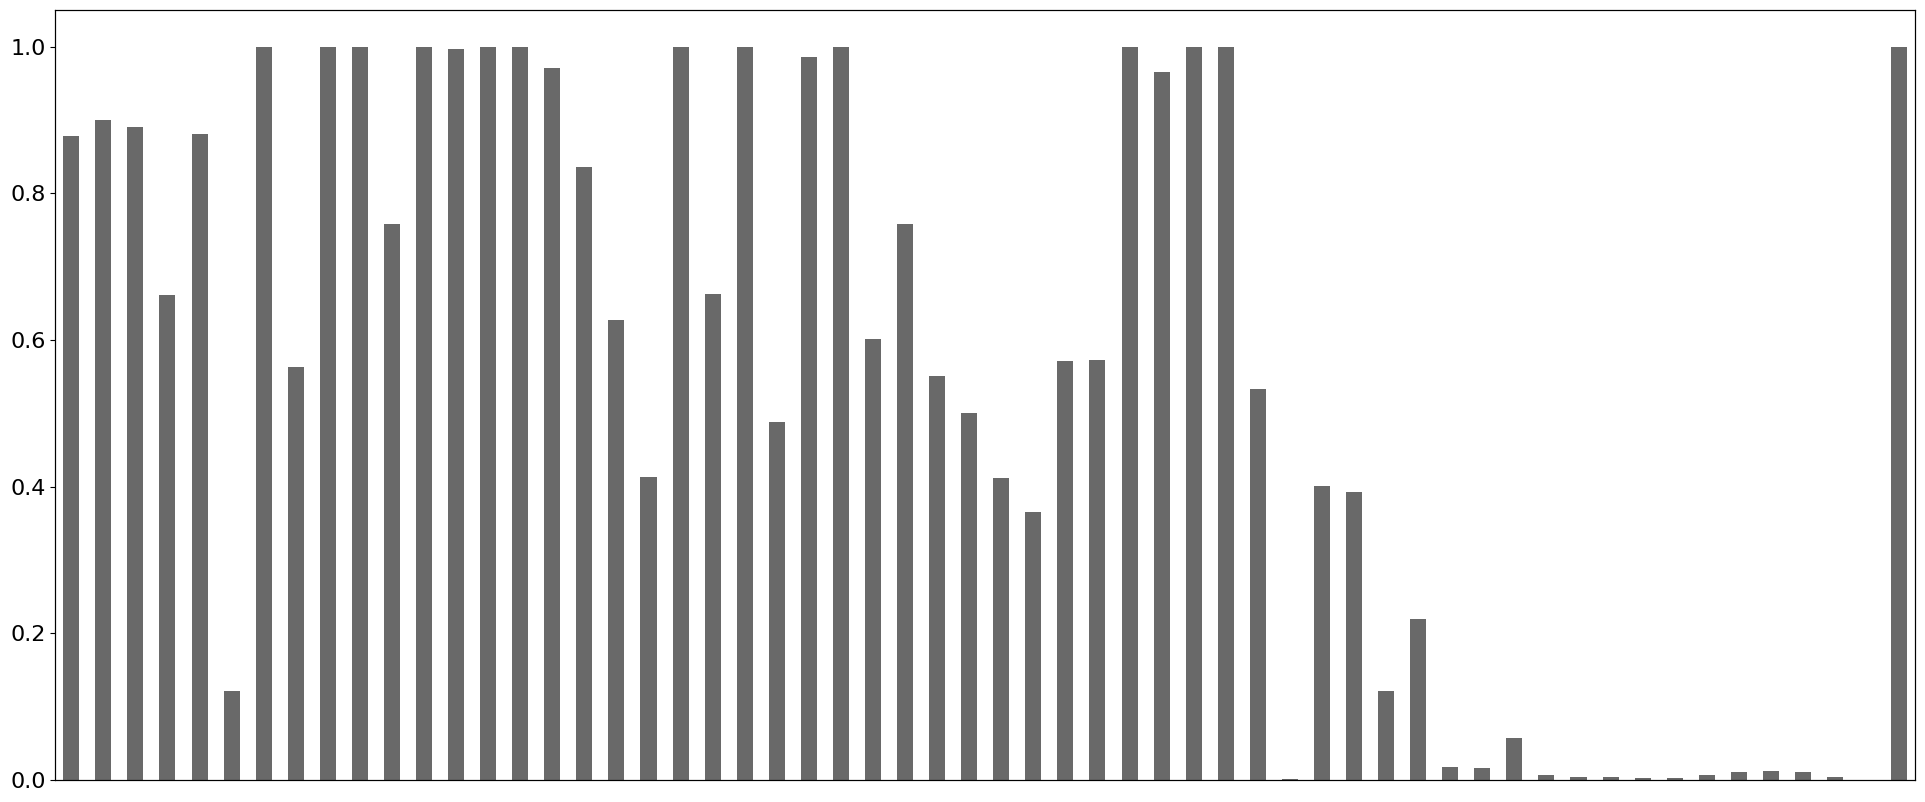
\includegraphics[width=1\linewidth]{priceprediction/data/null.png}
\caption{Histogram of non-null values in the scraped dataset across our features}
\end{figure}

Given this, we undertook an extensive removal process.

Effective data cleaning is crucial for ensuring the reliability and accuracy of our predictive model. The raw dataset contained several inconsistencies and irrelevant data points, which necessitated a thorough cleaning process. This section details the steps taken to clean the data, including the identification and removal of outliers, standardization of formats and types, and handling of missing values.

\subsection{Identifying and Removing Outliers}
\begin{enumerate}
    \item \textbf{Electric Vehicles}: Due to their really low number of appearances (1326) in our dataset, and also their specific price points, such as range, and battery capacity, we had to remove them completely.
    \item \textbf{Leasing Vehicles}: Vehicles listed under leasing agreements were also classified as outliers, being present in only 322 samples of such examples. The incomplete information on leasing terms and the difficulty in approximating their real prices led to their removal along with their specific columns.
    \item \textbf{Tuning}: Tuned cars were removed as they were considered outliers and lacked detailed information, which could vary significantly. We had only 482 such vehicles in our dataset.
\end{enumerate}

\subsection{Standardizing Data Formats}
\begin{itemize}
    \item \textbf{Price Data}: We decided to keep only prices that represent the EUR currency. Although the approach to convert the RON ones to their EUR equivalent seemed like the right decision at first glance, we detected some bad placed advertisement, that had their currency set to RON, but the price represented their actual EUR price. We remove 46 samples in total at this step.
    \item \textbf{Removing Error Prone Columns}: Columns with boolean values such as \textit{has vin (chassis number), vintage car, tuning, right-hand drive} where null values could not be assumed as False were removed to avoid introducing false negatives. 210 samples were removed.
\end{itemize}

\subsection{Handling Missing Values}
\begin{itemize}
    \item \textbf{Dropping Columns with High Null Values}: Due to a high number of null values, the following categories of columns were dropped: fuel consumption related, pollution related, and history related.
    \item \textbf{Selective Column Removal}: Certain columns from the general category, such as \textit{generation} and \textit{version}, were also removed due to their extremely sparse nature and high null appearances.
\end{itemize}

\subsection{Removing structured data outliers}
Although we previously removed several outliers from our dataset, such as electric vehicles and tuned cars, resulting in a more robust and complete dataset presented in \hyperref[tab:cleaned-table]{Table 3.2}, further analysis revealed that multiple key parameters still contained outliers. These outliers, if left unaddressed, could skew the results of our predictive model.

During our initial phases of data analysis, we identified several key metrics with significant outliers in terms of the number of samples. To ensure the robustness and accuracy of our model, we applied additional filtering criteria to remove these outliers, while still maintaining a good range of generalization.

\textbf{Power}: We filtered out vehicles with power greater than 600 HP or less than 50 HP. These values were deemed unrealistic for most vehicles in our dataset and would have introduced unnecessary noise into our model.

\begin{lstlisting}
df = df[df["power"] <= 600]
df = df[df["power"] >= 50]
# power: removed 218 rows
\end{lstlisting}

\textbf{Engine Capacity}: Vehicles with an engine capacity less than 500 cc or greater than 4000 cc were removed. This range was selected to exclude some badly placed advertisements, such as motorcycles, trucks, and other vehicles not representative of standard passenger cars.

\begin{lstlisting}
df = df[df["engine capacity"] >= 500]
df = df[df["engine capacity"] <= 4000]
# engine capacity: removed 305 rows
\end{lstlisting}

\textbf{Price}: We excluded vehicles with prices exceeding 40,000 EUR. These high-priced cars constituted a very small subset of our dataset and often included luxury or rare models that do not reflect general market trends. Additionally, buyers interested in such expensive cars typically rely on professional businesses for evaluation, making them outside the scope of our target market.

\begin{lstlisting}
df = df[df["price"] <= 40_000]
# price: removed 3911 rows
\end{lstlisting}

\textbf{Kilometers Driven}: Cars with more than 500,000 kilometers were removed, as they were also a small subset in our dataset.

\begin{lstlisting}
df = df[df["km"] <= 500_000]
# km: removed 30 rows
\end{lstlisting}

\textbf{Manufacturer Count}: We filtered out manufacturers with fewer than 100 listings in the dataset. Since the manufacturer and model are crucial factors in price prediction, brands with limited listings could skew the results due to insufficient data. By focusing on more common manufacturers, we create a more balanced and reliable dataset.

\begin{lstlisting}
temp_df = df["manufacturer"].value_counts()
df = df[df["manufacturer"].isin(temp_df[temp_df >= 100].index)]
# manufacturer: removed 482 rows
\end{lstlisting}

All these outliers are visually illustrated in \hyperref[fig:outliers]{Figure 3.3}.

\begin{figure}[ht]
    \centering
    \begin{subfigure}[b]{0.32\linewidth}
        \centering
        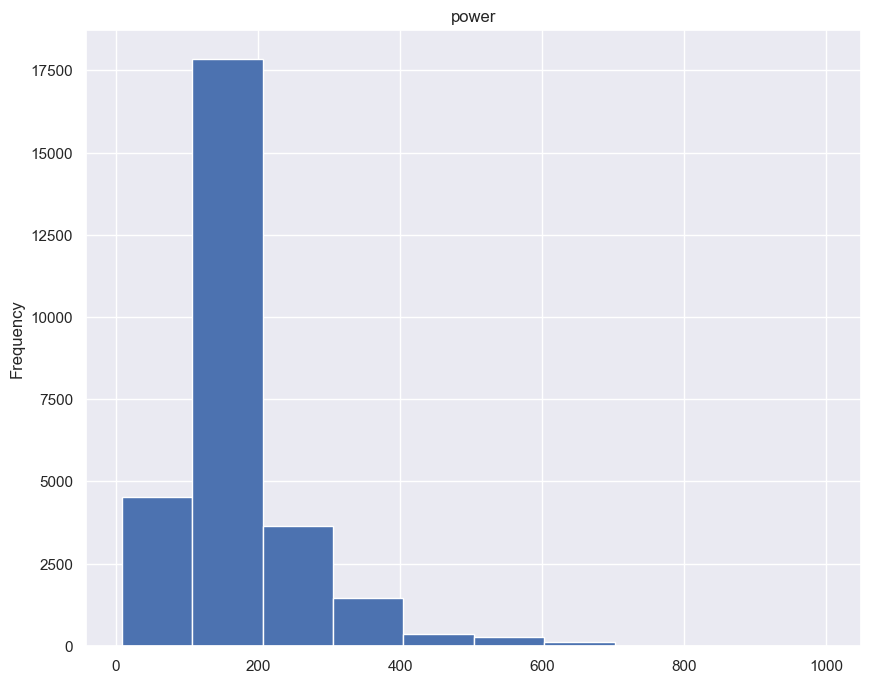
\includegraphics[width=\linewidth]{images/priceprediction/outliers/power.png}
        \caption{power}
        \label{fig:power}
    \end{subfigure}
    \hfill
    \begin{subfigure}[b]{0.32\linewidth}
        \centering
        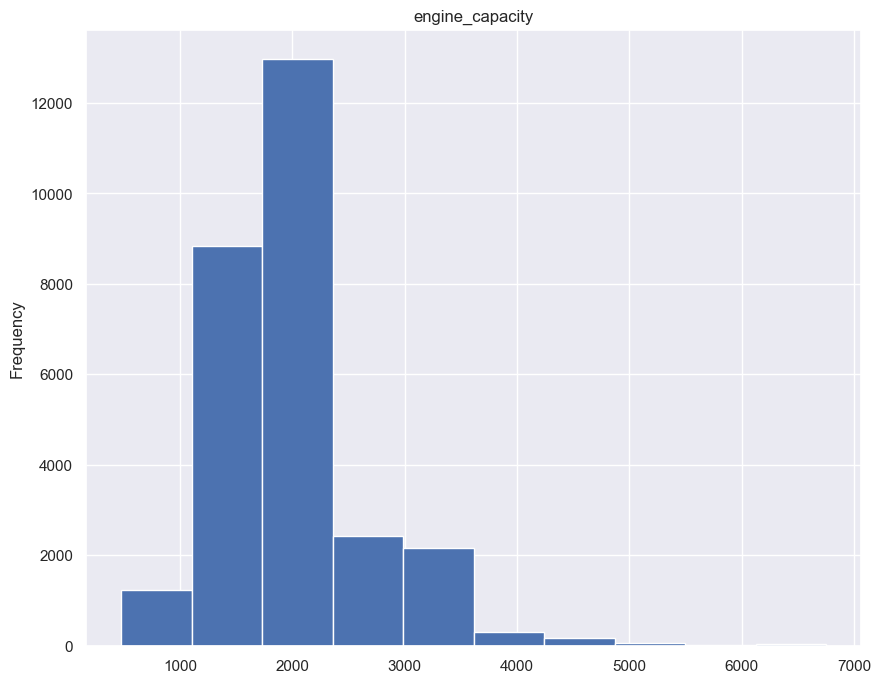
\includegraphics[width=\linewidth]{images/priceprediction/outliers/engine_capacity.png}
        \caption{engine\_capacity}
        \label{fig:engine_capacity}
    \end{subfigure}
    \hfill
    \begin{subfigure}[b]{0.32\linewidth}
        \centering
        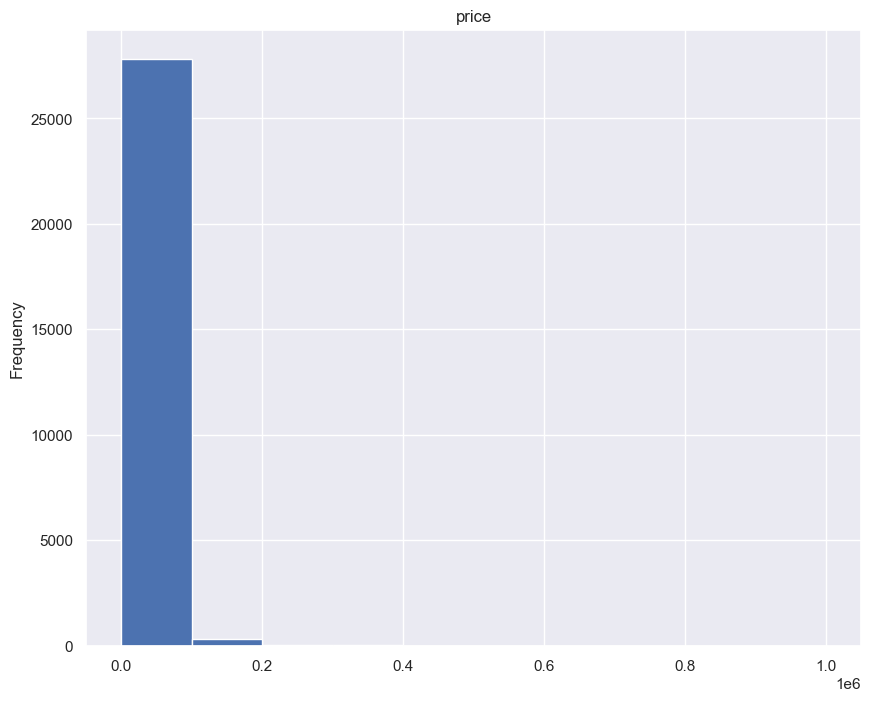
\includegraphics[width=\linewidth]{images/priceprediction/outliers/price.png}
        \caption{price}
        \label{fig:price}
    \end{subfigure}
    \vfill
    \begin{subfigure}[b]{0.48\linewidth}
        \centering
        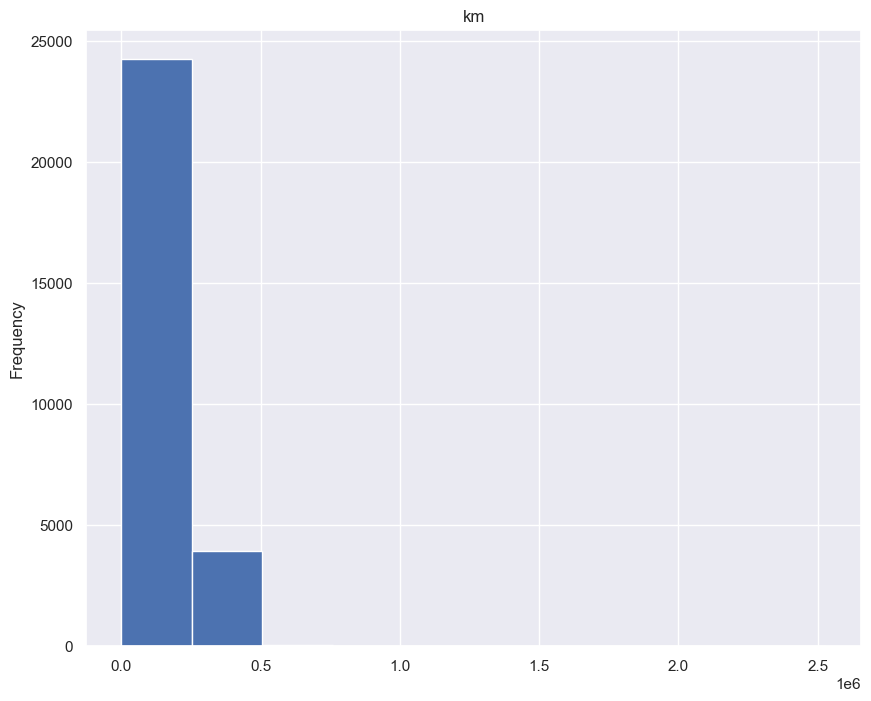
\includegraphics[width=\linewidth]{images/priceprediction/outliers/km.png}
        \caption{km}
        \label{fig:km}
    \end{subfigure}
    \hfill
    \begin{subfigure}[b]{0.48\linewidth}
        \centering
        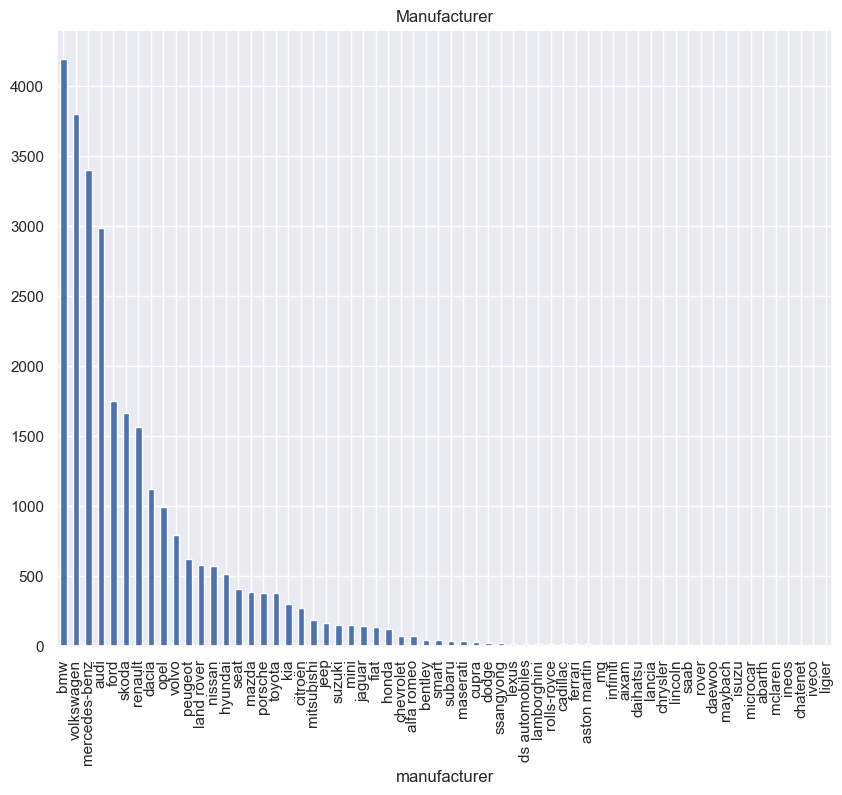
\includegraphics[width=\linewidth]{images/priceprediction/outliers/manufacturer.png}
        \caption{manufacturer\_count}
        \label{fig:manufacturer_count}
    \end{subfigure}
    \caption{Histograms of various features before filtering}
    \label{fig:outliers}
\end{figure}


\paragraph{The final structure of our dataset is presented in \hyperref[tab:cleaned-table]{Table 3.2}.}

\begin{longtable}{llll}
    \textbf{Column} & \textbf{Discrete/Continuous} & \textbf{Type} \\ \hline
    price & continuous & number \\ \hline
    manufacturer & discrete & text  \\ \hline
    model & discrete  & text \\ \hline
    year & continuous & number \\ \hline
    km & continuous & number \\ \hline
    power & continuous  & number \\ \hline
    engine capacity & continuous & number \\ \hline
    fuel & discrete & text \\ \hline
    chassis & discrete & text \\ \hline
    is\_automatic & discrete & boolean \\ \hline
    sold\_by\_company & discrete & boolean \\ \hline
    description & continuous & text \\ \hline
    \caption{Final Dataset Structure}
    \label{tab:cleaned-table}
\end{longtable}


\section{Data Analysis}
This section is divided into two subsections: structured data analysis and unstructured data analysis. Each subsection aims to provide a comprehensive understanding of the dataset by examining different types of data and extracting meaningful insights, while also validating our dataset.

\subsection{Structured Data}
In this subsubsection, we focus on analyzing the structured data, including both numerical and categorical variables. This analysis helps in understanding the distributions, relationships, and patterns within the dataset.

\subsubsection{Numerical Data Analysis}

\begin{itemize}
    \item \textbf{Price}: The histogram of car prices reveals a right-skewed distribution, with most cars priced between 5,000 and 15,000 EUR. This skewness indicates a higher concentration of lower-priced vehicles, which is typical for a second-hand car market.

    \begin{figure}[!h]
        \centering
        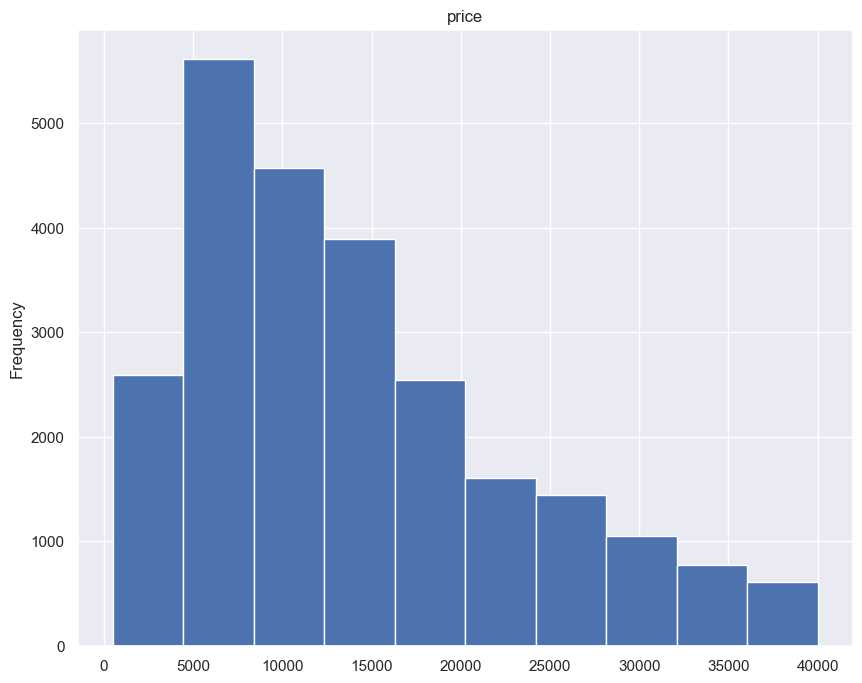
\includegraphics[width=0.5\linewidth]{images/priceprediction/after_outliers/price.png}
        \caption{Price Histogram}
        \label{fig:price-hist}
    \end{figure}

    \item \textbf{Year}: The year of manufacture is a critical factor in estimating a car's selling price. The histogram in \hyperref[fig:year-hist]{Figure 3.5 (a)} shows that most advertisements are for cars that are five to ten years old, with fewer listings for older vehicles. This reflects market trends favoring newer models. Additionally, the correlation between price and year of manufacture shown in \hyperref[fig:year-box]{Figure 3.5 (b)} aligns with real-world data, where newer cars typically command higher prices.
    
    \begin{figure}[ht]
        \begin{subfigure}[b]{0.48\linewidth}
            \centering
            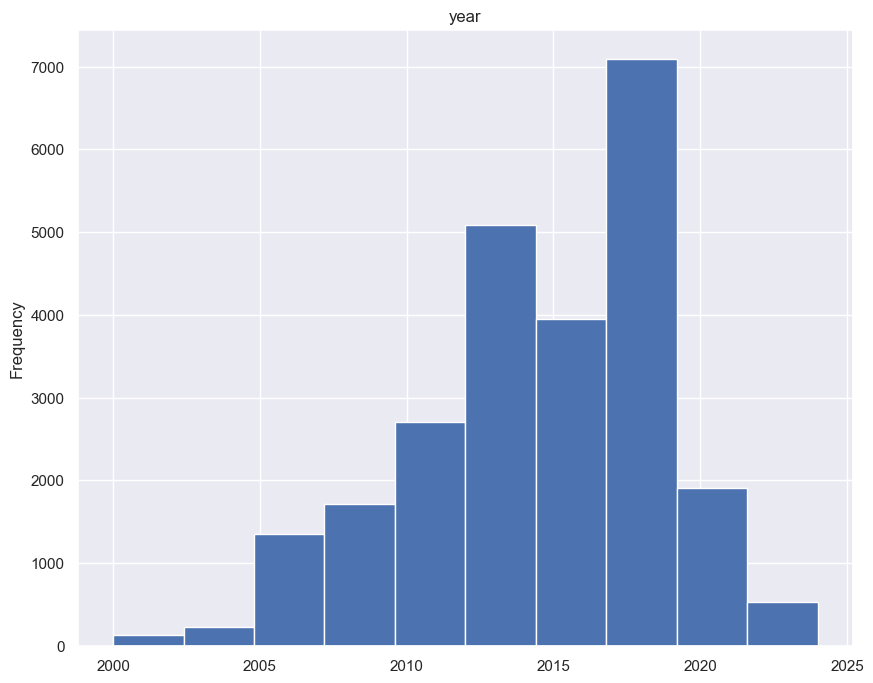
\includegraphics[width=\linewidth]{images/priceprediction/after_outliers/year.png}
            \caption{Year Histogram}
            \label{fig:year-hist}
        \end{subfigure}
        \hfill
        \begin{subfigure}[b]{0.48\linewidth}
            \centering
            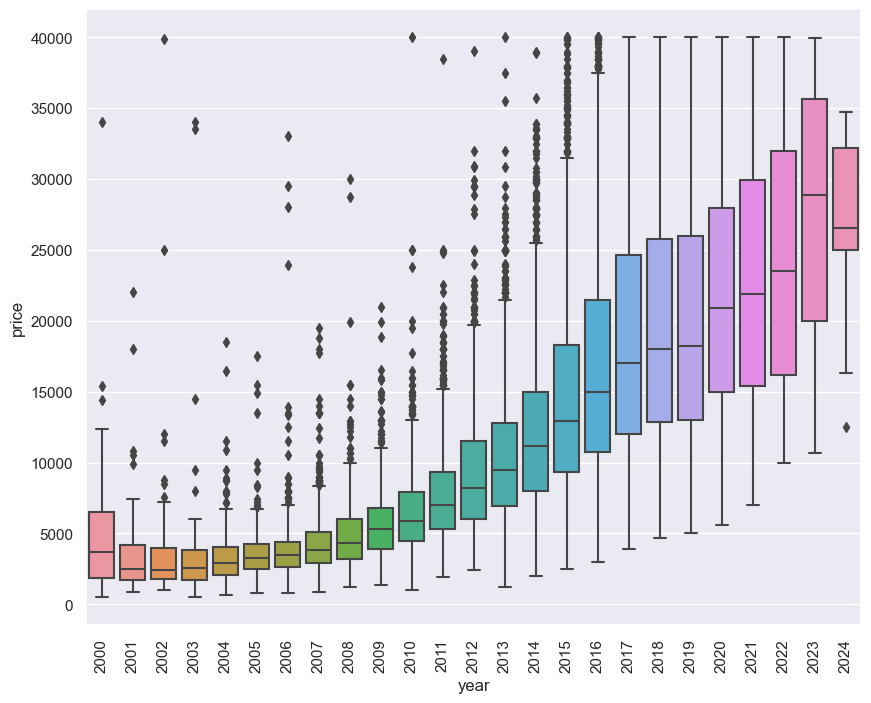
\includegraphics[width=\linewidth]{images/priceprediction/boxplots/year_price.png}
            \caption{Box plot price \& year}
            \label{fig:year-box}
        \end{subfigure}
        \caption{Year analysis}
        \label{fig:year}
    \end{figure}

     \item \textbf{Kilometers}: The distribution of kilometers driven, as shown in \hyperref[fig:km-hist]{Figure 3.6 (a)}, indicates that most cars have mileage between 100,000 and 250,000 kilometers. Higher mileage vehicles are less common, reflecting the typical lifespan of cars and their lower market value. This trend is observed in \hyperref[fig:km-box]{Figure 3.6 (b)}, where cars with higher mileage tend to be cheaper, aligning with the market preference for relatively low-mileage vehicles.

     \begin{figure}[!h]
        \begin{subfigure}[b]{0.48\linewidth}
            \centering
            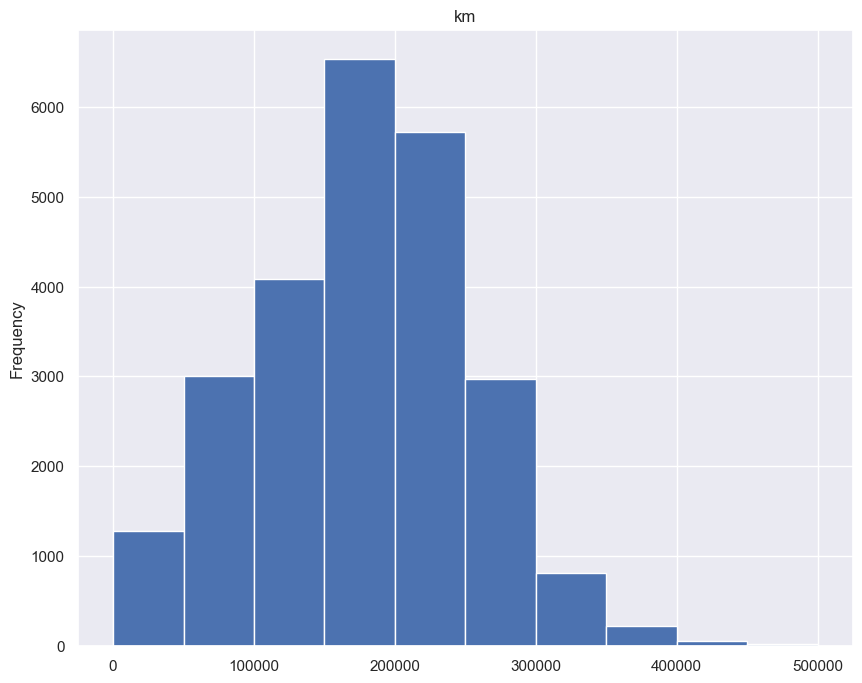
\includegraphics[width=\linewidth]{images/priceprediction/after_outliers/km.png}
            \caption{Kilometers Histogram}
            \label{fig:km-hist}
        \end{subfigure}
        \hfill
        \begin{subfigure}[b]{0.48\linewidth}
            \centering
            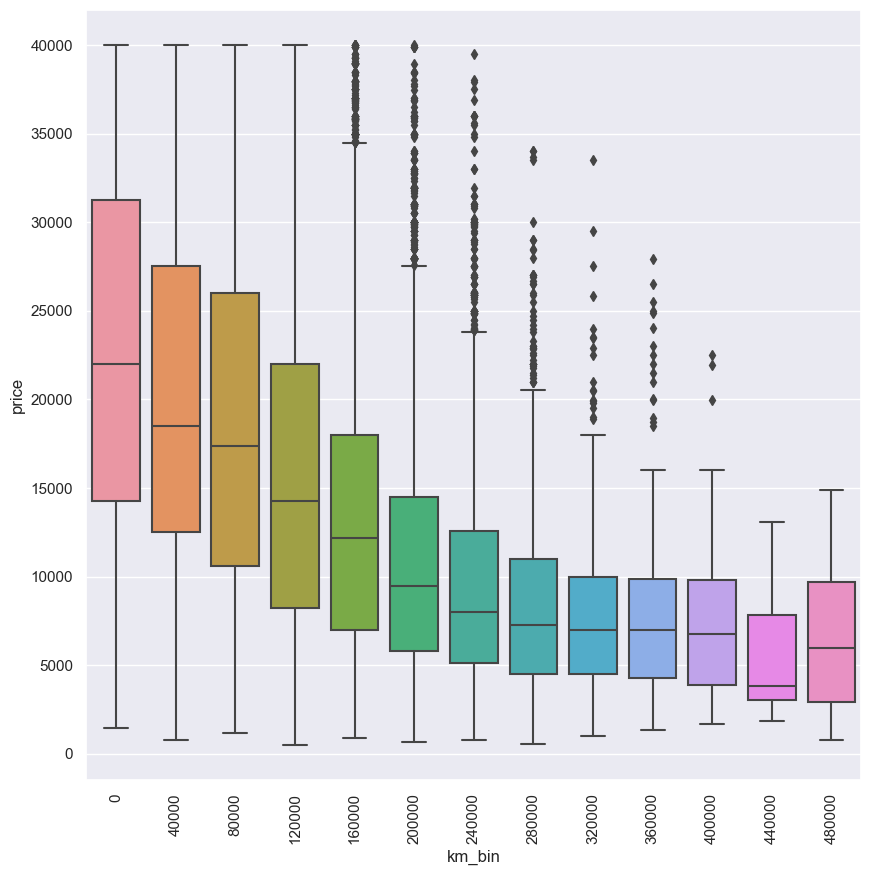
\includegraphics[width=\linewidth]{images/priceprediction/boxplots/km_price.png}
            \caption{Box plot price \& kilometers}
            \label{fig:km-box}
        \end{subfigure}
        \caption{Kilometers driven analysis}
        \label{fig:km}
    \end{figure}

    \item \textbf{Power and Engine Capacity}: Both power and engine capacity have a strong positive correlation with price. Higher power and larger engine capacity lead to higher selling prices due to their performance capabilities and appeal to buyers seeking more powerful vehicles, evidenced in \hyperref[fig:pow-eng-box]{Figure 3.7}.

    \begin{figure}[!h]
        \begin{subfigure}[b]{0.48\linewidth}
            \centering
            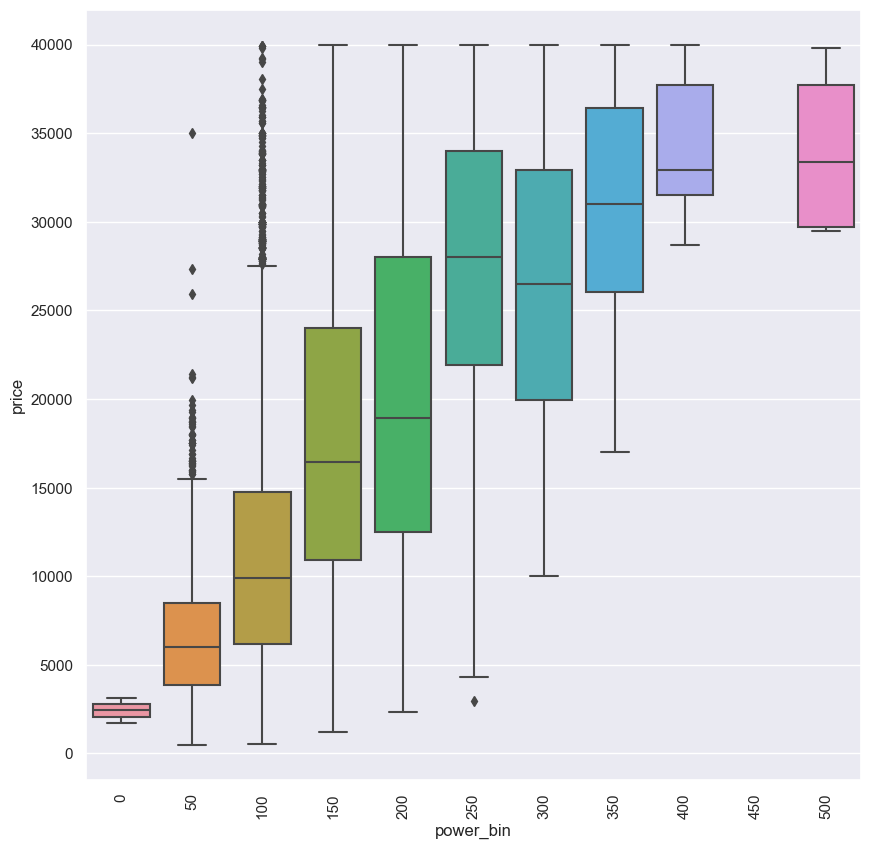
\includegraphics[width=\linewidth]{images/priceprediction/boxplots/power_price.png}
            \caption{Box plot price \& power}
            \label{fig:power-box}
        \end{subfigure}
        \hfill
        \begin{subfigure}[b]{0.48\linewidth}
            \centering
            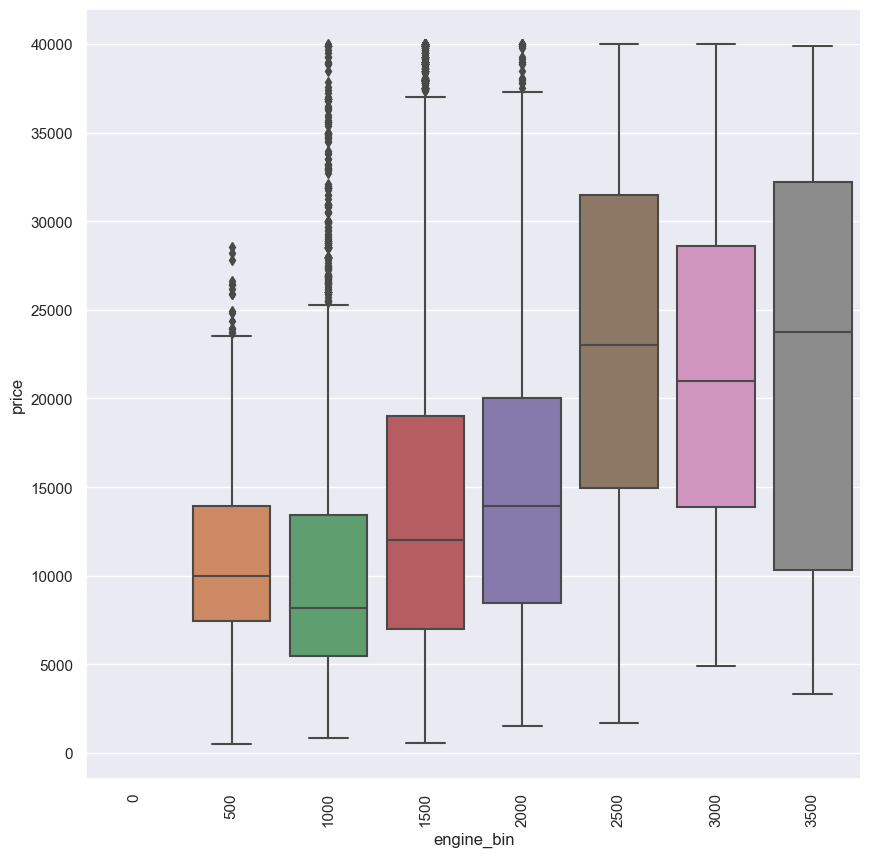
\includegraphics[width=\linewidth]{images/priceprediction/boxplots/engine_capacity_price.png}
            \caption{Box plot price \& engine\_capacity}
            \label{fig:eng-box}
        \end{subfigure}
        \caption{Power \& engine capacity analysis}
        \label{fig:pow-eng-box}
    \end{figure}
    
\end{itemize}

\subsubsection{Categorical Data Analysis}

\begin{itemize}
    \item \textbf{Manufacturer}: The bar chart in \hyperref[fig:manufacturer-hist]{Figure 3.8 (a)} illustrates the frequency of different car brands, with Volkswagen, BMW, and Audi being the most common. Additionally, the box plot in \hyperref[fig:manufacturer-box]{Figure 3.8 (b)} shows the relationship between manufacturers and prices, indicating that some brands, such as Mercedes, Porsche, and Volvo, tend to be pricier. This is expected, as these manufacturers primarily produce luxury vehicles, which command higher prices in the used cars market.

    \begin{figure}[!h]
        \begin{subfigure}[b]{0.48\linewidth}
            \centering
            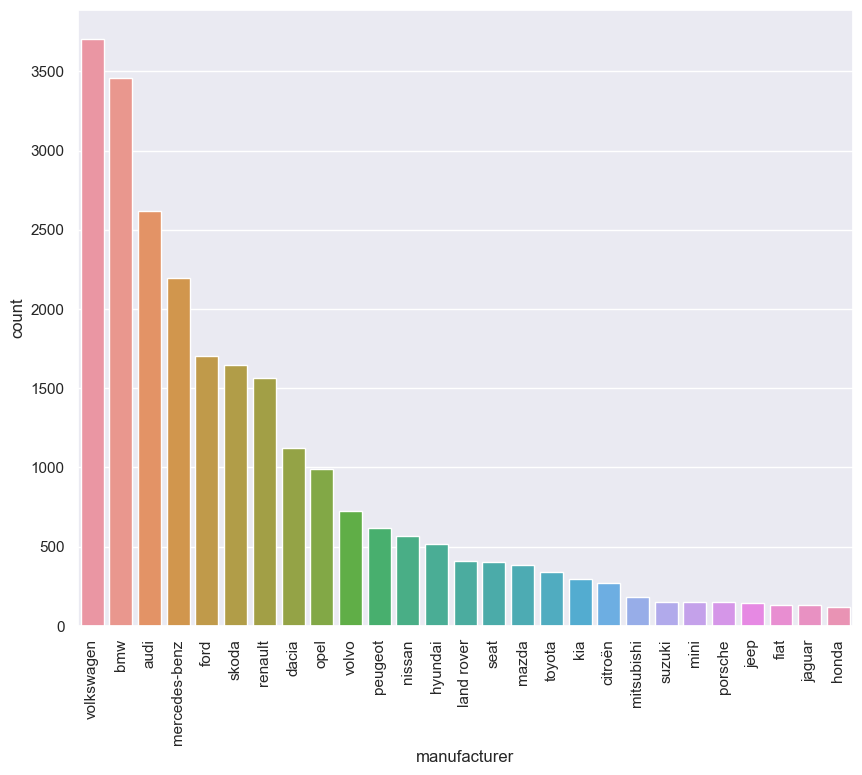
\includegraphics[width=\linewidth]{images/priceprediction/histograms/manufacturer-hist.png}
            \caption{Manufacturer Histogram}
            \label{fig:manufacturer-hist}
        \end{subfigure}
        \hfill
        \begin{subfigure}[b]{0.48\linewidth}
            \centering
            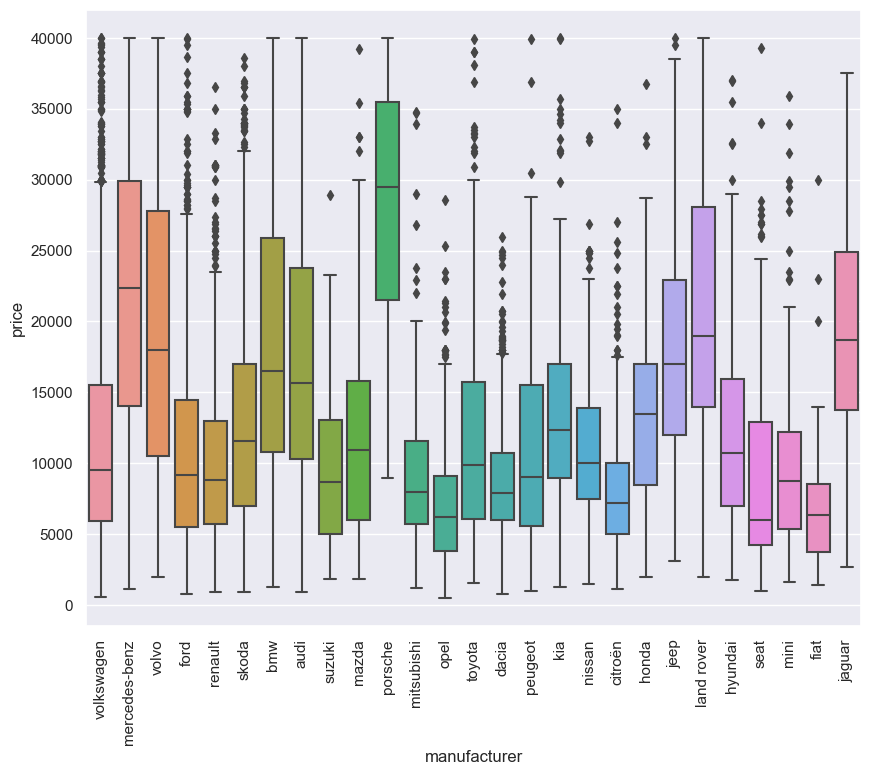
\includegraphics[width=\linewidth]{images/priceprediction/boxplots/manufacturer_price.png}
            \caption{Box plot price \& manufacturer}
            \label{fig:manufacturer-box}
        \end{subfigure}
        \caption{Manufacturer Analysis}
        \label{fig:manufacturer-analysis}
    \end{figure}
    
    \item \textbf{Fuel \& Chassis}: The correlation between fuel type and price, as well as chassis type and price, shown in \hyperref[fig:fuel-chassis-analysis]{Figure 3.9}, indicates that diesel cars are slightly more expensive, likely due to their renowned reliability. Additionally, coupes and SUVs tend to command higher prices compared to smaller city cars, owing to their more appealing and stately appearance.

    \begin{figure}[!h]
        \begin{subfigure}[b]{0.48\linewidth}
            \centering
            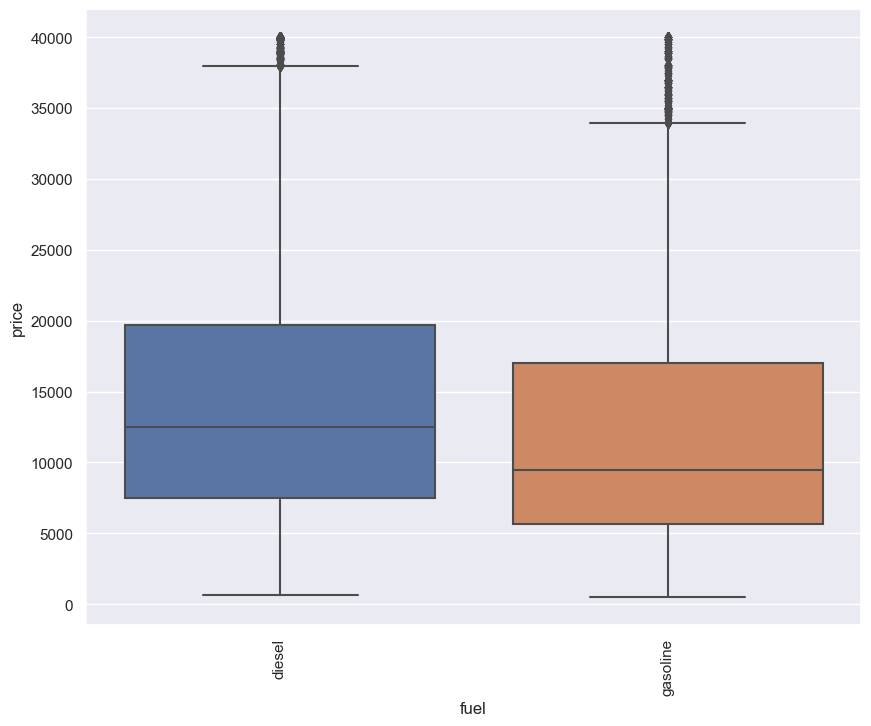
\includegraphics[width=\linewidth]{images/priceprediction/boxplots/fuel_price.png}
            \caption{Box plot price \& fuel}
            \label{fig:fuel-box}
        \end{subfigure}
        \hfill
        \begin{subfigure}[b]{0.48\linewidth}
            \centering
            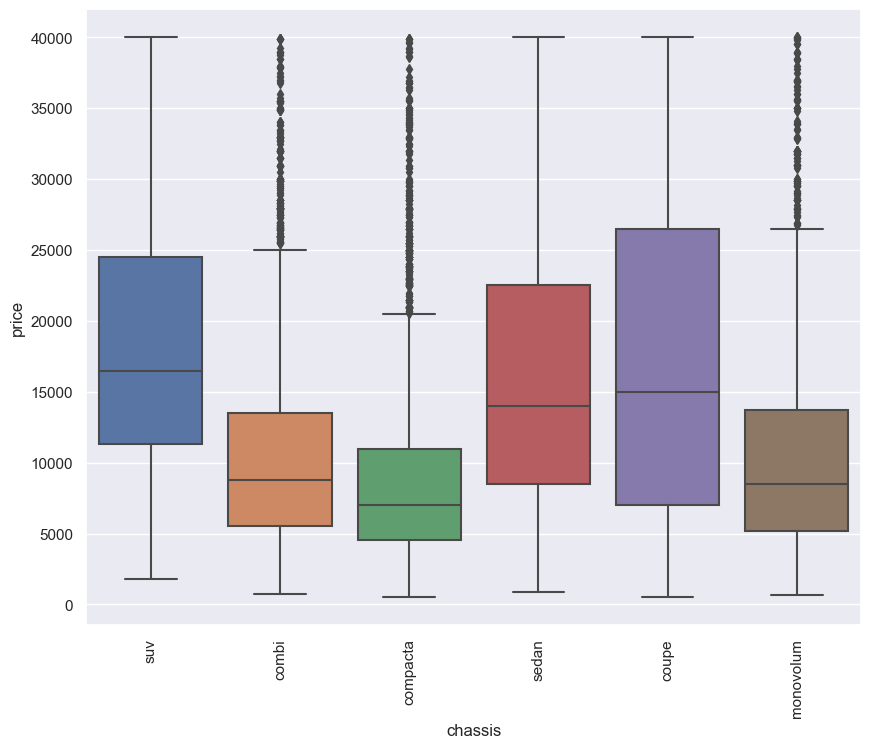
\includegraphics[width=\linewidth]{images/priceprediction/boxplots/chassis_price.png}
            \caption{Box plot price \& chassis}
            \label{fig:chassis-box}
        \end{subfigure}
        \caption{Fuel \& Chassis Analysis}
        \label{fig:fuel-chassis-analysis}
    \end{figure}

    \item \textbf{Gearbox \& Seller}: In \hyperref[fig:gearbox-seller-analysis]{Figure 3.10}, there is a clear relationship between gearbox type and price, with automatic cars fetching higher resale prices due to the comfort they provide. Furthermore, cars sold by businesses are generally priced higher, as these sellers include their profit margins in the resale price.

    \begin{figure}[!h]
        \begin{subfigure}[b]{0.48\linewidth}
            \centering
            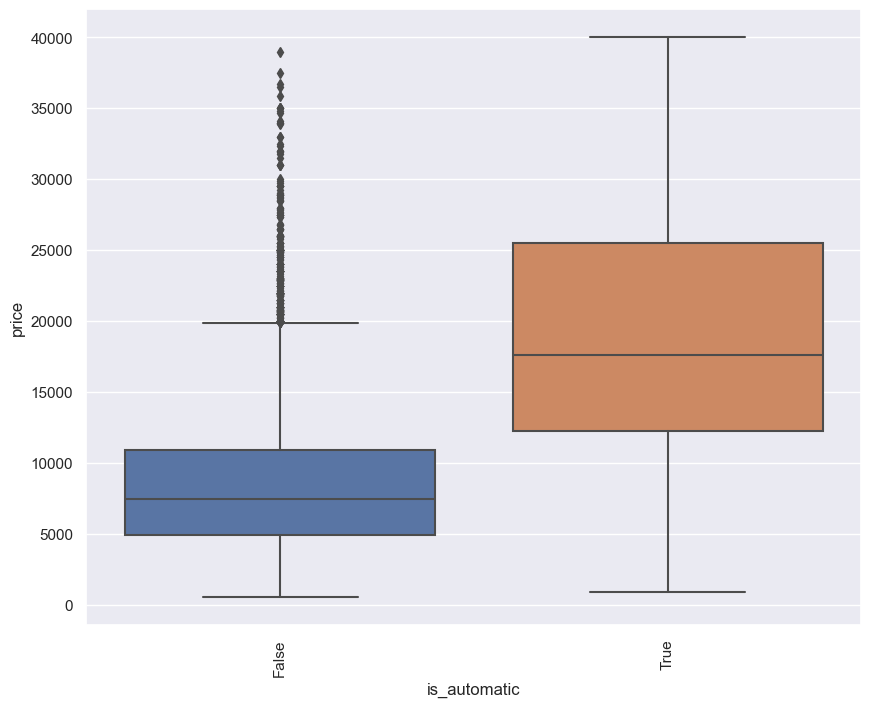
\includegraphics[width=\linewidth]{images/priceprediction/boxplots/is_automatic_price.png}
            \caption{Box plot price \& gerabox}
            \label{fig:gearbox-box}
        \end{subfigure}
        \hfill
        \begin{subfigure}[b]{0.48\linewidth}
            \centering
            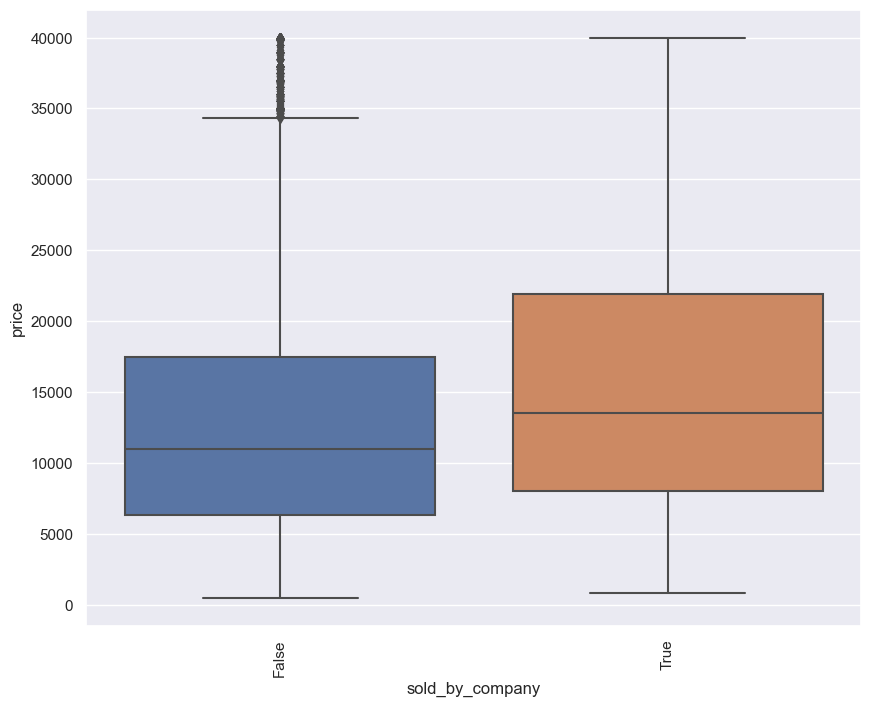
\includegraphics[width=\linewidth]{images/priceprediction/boxplots/sold_by_company_price.png}
            \caption{Box plot price \& seller}
            \label{fig:seller-box}
        \end{subfigure}
        \caption{Gearbox \& Seller Analysis}
        \label{fig:gearbox-seller-analysis}
    \end{figure}
    
\end{itemize}

\subsection{Unstructured Data}
This subsection focuses on the analysis of unstructured data, including text descriptions and images. These analyses complement the structured data insights and provide a more holistic understanding of the dataset.


\subsubsection{Image Data Analysis}

The analysis of images was conducted manually, primarily observing the following aspects:

\begin{itemize}
    \item In the images resulting from the scraping process, we failed to identify a pattern in the angles from which the photos were taken. While advertisements posted by companies tend to have more professional photos, as showcased in \hyperref[fig:sample-images]{Figure 3.11}, the ones posted by normal users have various formats. We've conducted manual selection, trying to select similar angles throughout our dataset by selecting front-to-side pictures for each sample. Luckily, our decision to scrape ten images for each entry gave us a big enough selection pool to achieve this.
    \item Some company-posted advertisements include banners, as seen in \hyperref[fig:sample-images]{Figure 3.11}, which could confuse our feature extraction model. This issue was also mitigated by manually selecting one image per sample without such banners.
\end{itemize}

\begin{figure}[ht]
    \centering
    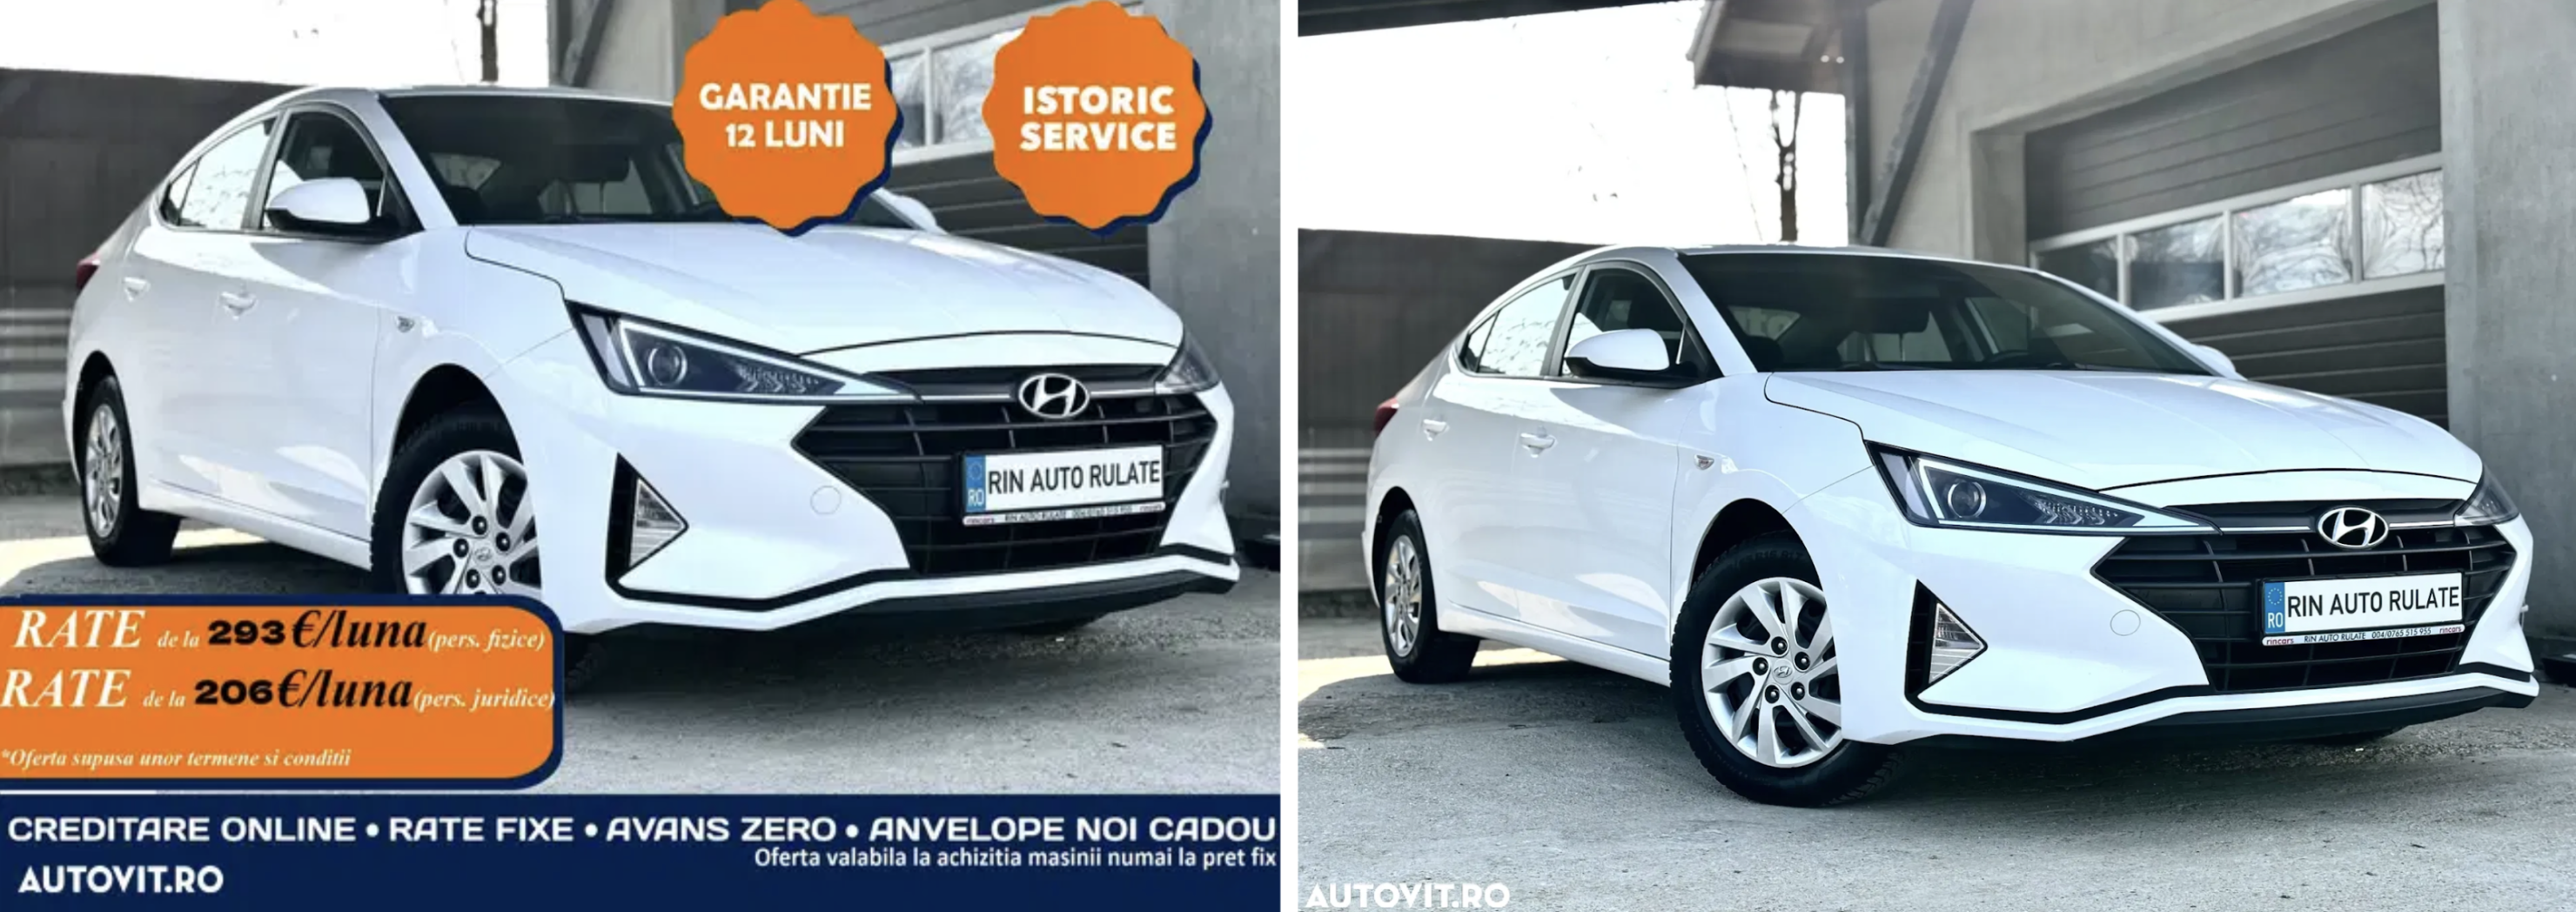
\includegraphics[width=1\linewidth]{images/priceprediction/data/Screenshot 2024-05-28 at 21.33.30.png}
    \caption{Sample Images}
    \label{fig:sample-images}
\end{figure}

\subsubsection{Text Data Analysis}

For the analysis of the descriptions, we conducted both programmatic and manual analyses.

During our manual analysis, we observed a significant issue: some advertisements were posted in languages other than Romanian. This discrepancy would have greatly affected our model, as we are using a BERT model pre-trained and specialized in Romanian.

To address this, we employed the \textit{langdetect} library \cite{langdetect} to detect the language of each description. After identifying foreign language samples, we carefully removed them from our dataset. \autoref{lst:langs} shows the detected languages and their frequency.

\begin{lstlisting}[label={lst:langs}]
{'ro': 23964, 'it': 478, 'en': 228, 'ca': 7, 'de': 1, 'sl': 1, 'id': 2, 'pt': 2, 'af': 1, 'sv': 1, 'fr': 1, 'et': 1}
\end{lstlisting}

We also found that many descriptions contained email addresses, phone numbers, URLs, HTML tags such as <strong>, and a surprisingly large number of emojis. Since these elements do not provide any value to our regression model, we removed them using regular expressions. For emojis, we utilized the \textit{emoji} \cite{emoji} package from pip.

\begin{listing}[H]
\begin{lstlisting}
def replace_patterns(text: str):
    email_pattern = r'\b(([^<>()\[\]\\.,;:\s@"]+(\.[^<>()\[\]\\.,;:\s@"]+)*)|(".+"))@((\[[0-9]{1,3}\.[0-9]{1,3}\.[0-9]{1,3}\.[0-9]{1,3}])|(([a-zA-Z\-0-9]+\.)+[a-zA-Z]{2,}))\b'
    phone_pattern = r"\b^[\+]?[(]?[0-9]{3}[)]?[-\s\.]?[0-9]{3}[-\s\.]?[0-9]{4,6}$\b"
    url_pattern = r"https?:\/\/(www\.)?[-a-zA-Z0-9@:%._\+~#=]{1,256}\.[a-zA-Z0-9()]{1,6}\b([-a-zA-Z0-9()!@:%_\+.~#?&\/\/=]*)"
    soup = bs4.BeautifulSoup(text, "lxml")
    text = re.sub(email_pattern, "", text)
    text = re.sub(phone_pattern, "", text)
    text = re.sub(url_pattern, "", text)
    text = soup.get_text(text)
    text = emoji.replace_emoji(text, "")
    return text
\end{lstlisting}
\end{listing}

Additionally, the word cloud in \hyperref[fig:wordcloud]{Figure 3.12} shows frequently occurring terms in car descriptions, such as "airbag", "parking sensors", "abs", and "esp". These terms provide valuable context for our model and represent the expected result, as they are keywords from custom options and equipment.

\begin{figure}[ht]
    \centering
    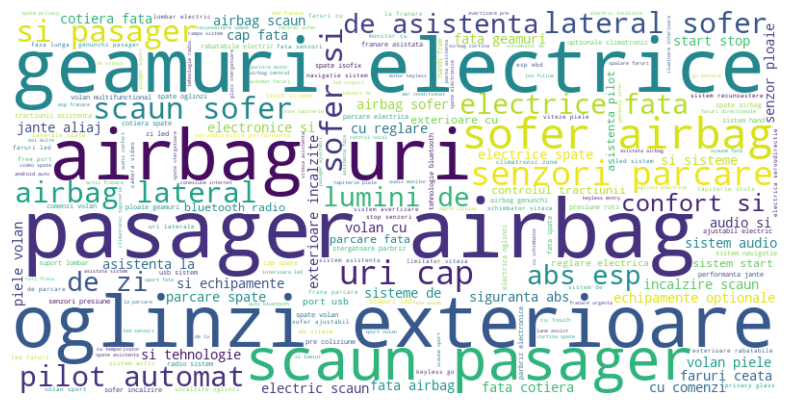
\includegraphics[width=\linewidth]{images/priceprediction/data/wordcloud.png}
    \caption{Descriptions Wordcloud}
    \label{fig:wordcloud}
\end{figure}


\subsubsection{Conclusion}
Our data analysis yielded valuable insights and a deep understanding of the dataset we scraped. We identified the key features that significantly impact car prices among our structured and numerical variables, validating our dataset by reflecting real-world market trends. Additionally, this analysis allowed us to preemptively identify potential issues, enabling us to focus more effectively on optimizing our model. These findings underscore the robustness of our dataset and provide a strong foundation for developing an accurate and reliable predictive model.
